Transaction throughput is a key benchmark for the performance of transactional
databases. Systems with stronger isolation levels tend to have lower transaction
throughput resulting from the increased number of aborted transactions.
Therefore, in this experiment, transaction throughput is used to determine the
performance impact of serializability in NVRAM-based key-value stores.

\subsubsection{Setup}

\todo[inline]{Make this a subsection (convert important paragraphs to subsubsections)}

\todo[inline]{Fix data IS vs data ARE inconsistency}

In order to perform this experiment, one not only needs data to work on but also
a set of concrete transactions and the operations they are composed of, i.e. a
workload. As with data, it is hard to acquire actual transaction traces and
determine their relevance. For that reason, the experiment setup relies heavily
on randomly generated data. However, each random choice is reproducible as the
generated data are stored on disk prior to the experiment. Hence, the only
non-deterministic behaviour is induced by multi-threading, the operating system,
and the underlying hardware.

\paragraph{Data}

The data used in the experiment comprise two distinct sets of randomly generated
key-value pairs. The first data set contains 1K pairs, whereas the second holds
100K entries. Lacking insights on meaningful layouts of key-value pairs, this
evaluation relies on the same layout used in \cite{bailey2013exploring}.
Accordingly, keys are 128-byte random strings and values are 1024-byte random
strings. When the experiment starts, each individual KVS is populated with these
key-value pairs.

% For uniformity, this experiment uses the exact same sets of random key-value
% pairs that are used in Chapter \ref{ch:eval-baseline}. Thus, there is one data
% set with 1K entries and another with 100K entries. When the experiment starts,
% each individual KVS will be populated with these key-value pairs.

\paragraph{Workloads}

All transactions that are to be executed during the experiment are encoded as a
workload. A workload specifies for each transaction its operations and the
respective key-value pairs to operate on. When generating a workload, there are
three important dimensions:

\begin{itemize}
    \item length of transactions
    \item number of transactions
    \item relative distribution of operations
\end{itemize}

The length of a transaction is the number of operations enclosed in that
transaction. Intuitively, the length of transactions should vary. Unfortunately,
no reliable sources as to the absolute quantities of transaction lengths could
be found. As a result, the following ranges are deemed meaningful:

\begin{figure}[!h]
    \centering
    \begin{tabular}{|l|l|l|}
        \hline
        \textbf{Name} & \textbf{Min. No. Ops} & \textbf{Max. No. Ops} \\
        \hline
        Short         & 2  & 32  \\
        Long          & 64 & 256 \\
        \hline
    \end{tabular}
    \caption{Types of transactions in terms of length.}
    \label{tab:tx-length}
\end{figure}

Short transactions can be small updates like incrementing a numeric value,
optionally based a small aggregation. Long transaction on the other hand, can be
larger aggregations such as computing a sum over many items.

When specifying the operations of a transaction, it must be decided whether an
operation reads or updates an item. Insert and delete operations are omitted as
they complicate the experiment when run concurrently. For example, a concurrent
transaction might fail because an expected pair has not been inserted yet. Such
an incident reduces transaction throughput without an actual conflict which
could distort results. The remaining two operations are selected based on the
empirical analysis in \cite{andrei2017sap}. According to the source, read
operations amount of 84\% of all operations. The remaining 16\% are sumsumed as
updates for this experiment. Each operation acts on keys from the dummy set that
are selected randomly during the workload generation. All pseudo-random numbers
were generated using uniform distributions based on seperate mersenne twister
engines. Each workload consists of 1000 transactions.

\paragraph{Scenarios}

Resulting from the dimensions shown above, four unique scenarios  were derived:

\begin{itemize}
    \item S1: small database, short transactions
    \item S2: small database, long transactions
    \item S3: large database, short transactions
    \item S4: large database, long transactions
\end{itemize}

These scenarios are supposed to simulate both low and high contention in
different forms. In a database that is small compared to the number of
concurrent transactions, it is very likely that multiple transactions operate on
the same data which can cause conflicts. Likewise, longer transactions cause
contention as they are more likely to access data of other transactions. That
said, scenario 1 and especially scenario 2 simulate high contention which is the
worst-case for any concurrency control. The reason is that contention often
causes conflicts which lead to aborts and reduced transaction throughput. With
larger databases, short transactions are less likely to access the same data
which reduces contention. However, as transactions become longer, they become
more likely to collide and abort.

\subsubsection{Procedure}

The benchmark is performed separately for each KVS. The general procedure is to
execute each workload with a different number of cores. Since the underlying
machine has 32 physical cores, the experiment is performed with 1, 2, 4, 8, 16,
and 32 cores. During each run, several statistics such as the total time taken
and the number of aborts are captured. In order to reduce the influence of
outliers, each run, i.e. a combination of workload and core count, is performed
10 times. As a result, for each store there is a total of 24 configurations
which amounts to a total of 480 runs including repetitions.

A single run of the benchmark works as follows. At first, the respective KVS is
initialized with dummy data and the workload decomposed so that it fits the
number of cores of the current configuration. Then, for each core, a thread is
created and pinned to that core. Each thread executes an equal share of the
entire workload. The total time taken to execute the entire workload is measured
by taking the difference of timestamps from before spawning the workers and
after all workers have terminated. The general procedure of the experiment is
depicted in Figure~\ref{fig:eval-host}. The procedure performed by a single
worker thread is shown in Figure~\ref{fig:eval-worker}.

\todo[inline]{Mention retry policy?}

\begin{figure}[h!]
\begin{minipage}[l]{0.50\textwidth}
    % 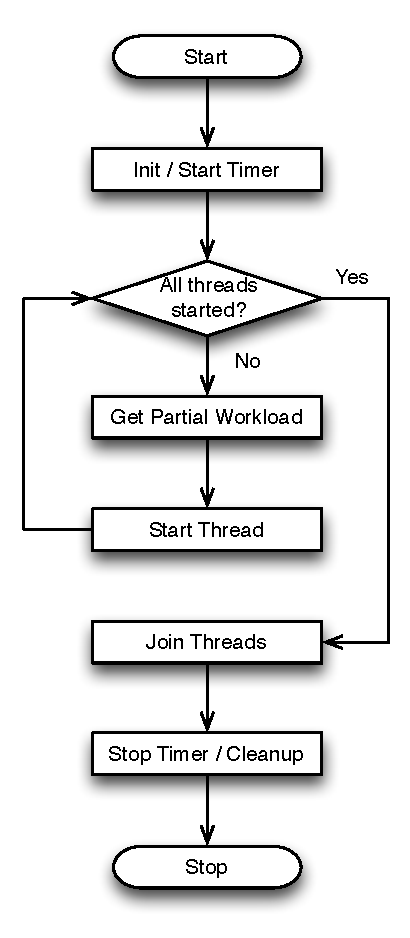
\includegraphics[width=0.85\textwidth]{figures/bench/host}
    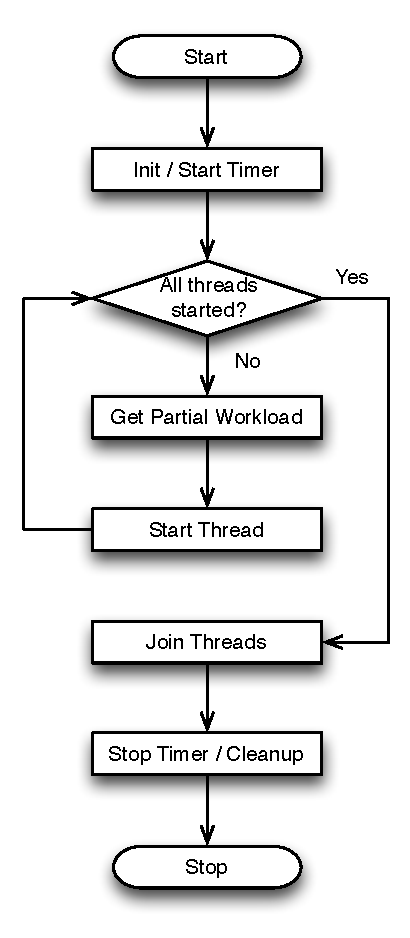
\includegraphics[width=0.75\textwidth]{figures/bench/host}
    \caption{Logical flow of the benchmark application.}
    \label{fig:eval-host}
\end{minipage}
\begin{minipage}[l]{0.50\textwidth}
    % 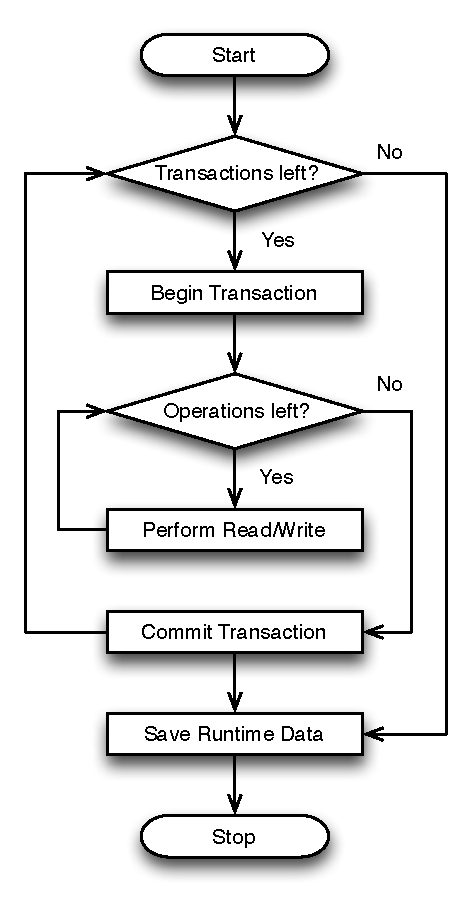
\includegraphics[width=\textwidth]{figures/bench/worker}
    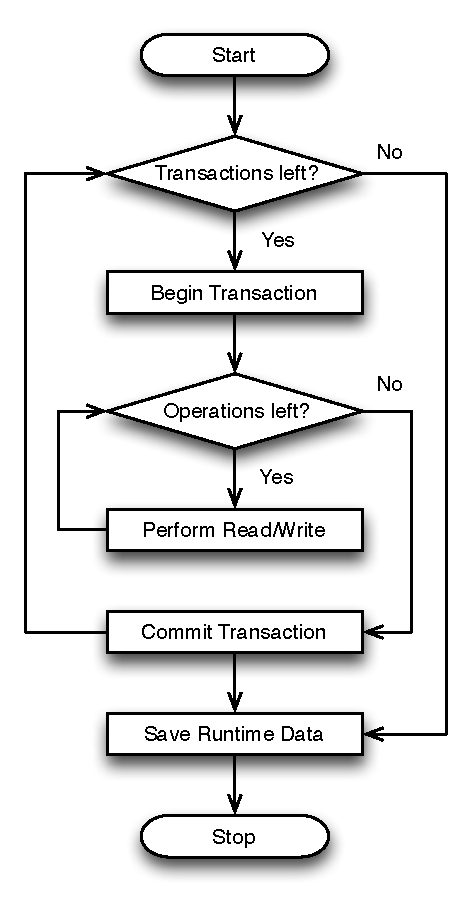
\includegraphics[width=0.89\textwidth]{figures/bench/worker}
    \caption{Logical flow of a single worker thread.}
    \label{fig:eval-worker}
\end{minipage}
\end{figure}

\subsubsection{Results \& Discussion}

\todo[inline]{Integrate raw ttp and parallel efficiency}

In this subsection the results of the benchmark are shown and discussed. The
benchmark captures two metrics: transaction throughput and the transaction abort
rate. In order to express the scalability of both KVS, throughput is expressed
in terms of speedup factor. This also helps comparing the performance of both
stores even if absolute throughput differs significantly. The abort rate is
given by the ratio of the number of aborted transactions and the number of
scheduled transactions. When interpreting throughputs and speedup factors, it is
important to take the abort rate into account because higher abort rates can
lead to higher transaction throughputs. The reason for this circumstance is that
commits are very expensive and the resulting time saving of an abort has a
stronger influence on throughput than reducing the number of committed
transactions. This is also a direct consequence of the two-level store
architecture and the additional measures to preserve consistency in NVRAM.

\paragraph{Legend}

The following analysis compares benchmark results of Echo (green), Midas (blue)
and an optimized variant of Midas (red). In the current implementation of Midas,
the index is based on a naive hash table implementation for NVRAM. In order to
protect critical sections in the hash table, a simple global locking mechanism
is used. This approach forms a major bottleneck which can be addressed with a
designated but often complicated concurrent design as in \cite{fan2013memc3}.
However, this is an implementation detail, albeit crucial. In order to show the
potential of Midas' design, a second variant of Midas without index locking was
examined. This is possible because during the benchmark not the index but only
histories are modified. This is a side effect of omitting insert and delete
operations for simplicity.

%==============================================================================
% [1 = SS]
%==============================================================================

\paragraph{Scenario S1}

This scenario simulates high contention through a small database. The plot in
Figure \ref{fig:ttp-s1} shows that both variants of Midas have a much better
transaction throughput than Echo. However, when considering the speedup factors
in Figure \ref{fig:spd-s1}, all stores fail to improve beyond a core count of
eight. This can also be seen in terms of parallel efficiency in Figure
\ref{fig:eff-s1}. The reason is that the database has very few items which
increases both synchronization overhead and the number of data conflicts. The
latter is reflected in an increased abort rate as shown in Figure
\ref{fig:ar-s1}. As expected, both variants of Midas have much higher abort
rates, due to stricter conflict detection. While Midas$^{*}$ makes better use of
additional cores, it also produces higher abort rates. This confirms the
implicit serializing nature of the global lock in the original implementation of
Midas.

\begin{figure}[h!]
\begin{minipage}[l]{0.50\textwidth}
    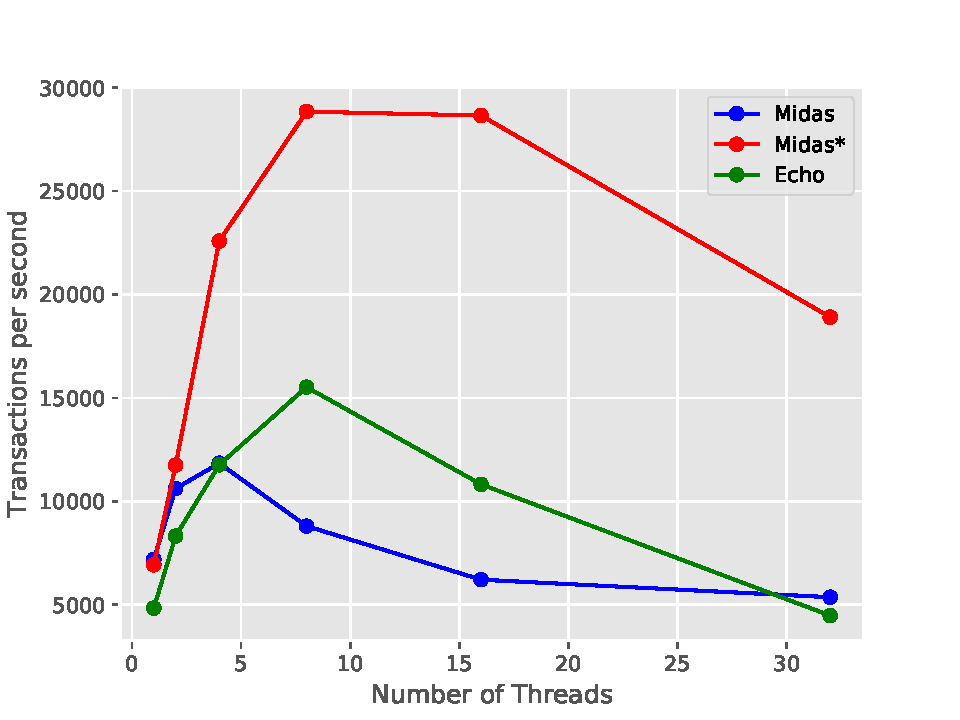
\includegraphics[width=\textwidth]{figures/bench/ttp-ss}
    \caption{Transaction throughput for\\scenario S1.}
    \label{fig:ttp-s1}
\end{minipage}
\begin{minipage}[l]{0.50\textwidth}
    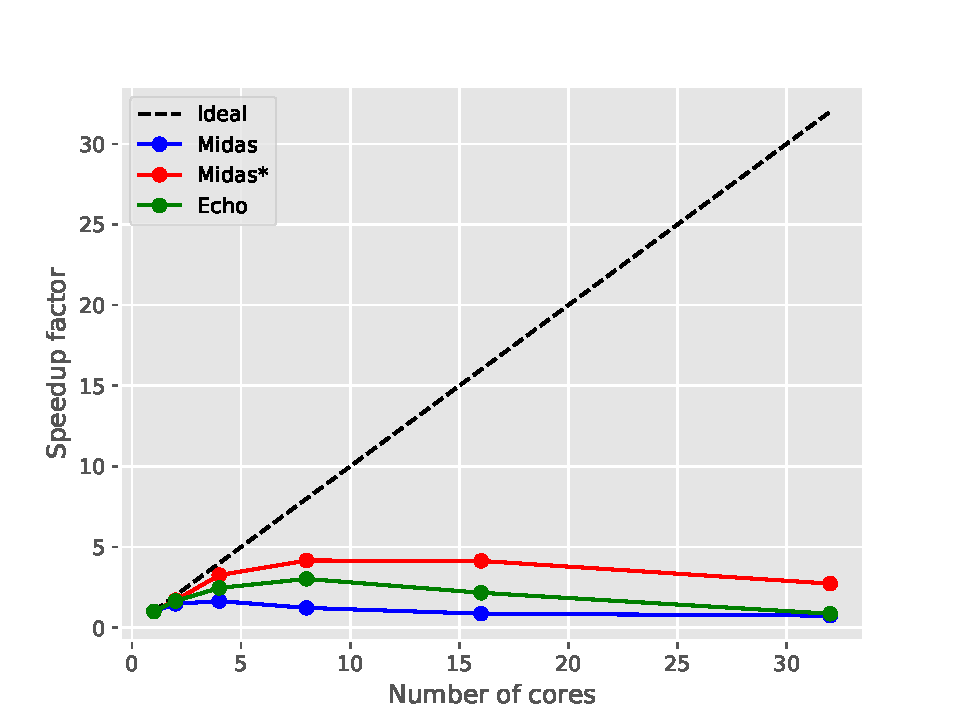
\includegraphics[width=\textwidth]{figures/bench/spd-ss}
    \caption{Transaction throughput speedup for scenario S1.}
    \label{fig:spd-s1}
\end{minipage}
\begin{minipage}[l]{0.50\textwidth}
    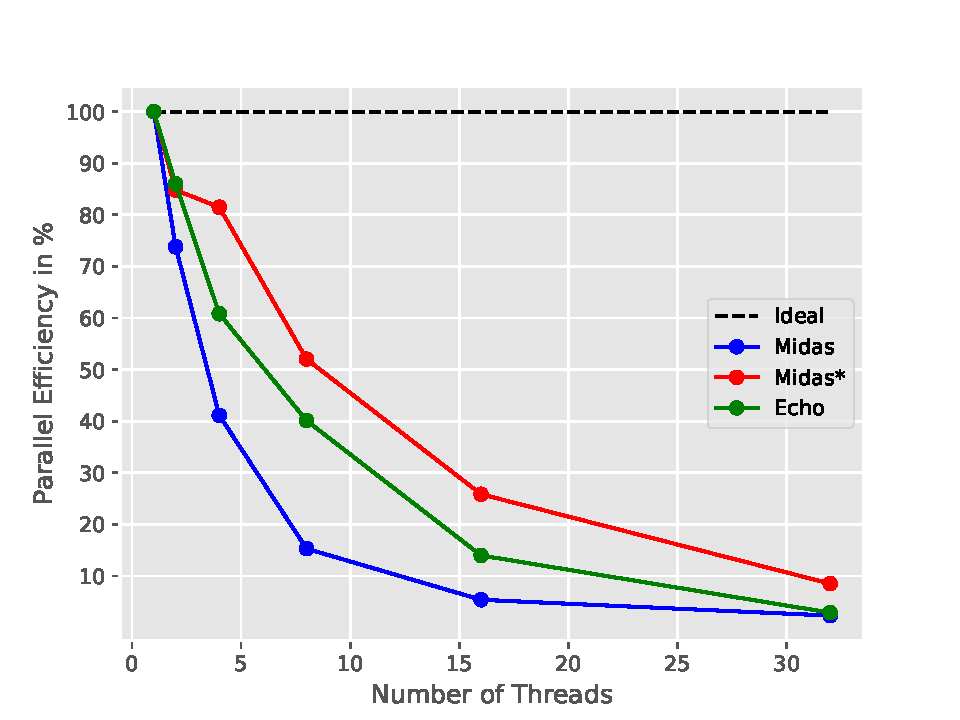
\includegraphics[width=\textwidth]{figures/bench/eff-ss}
    \caption{Parallel efficiency for scenario S1.}
    \label{fig:eff-s1}
\end{minipage}
\begin{minipage}[l]{0.50\textwidth}
    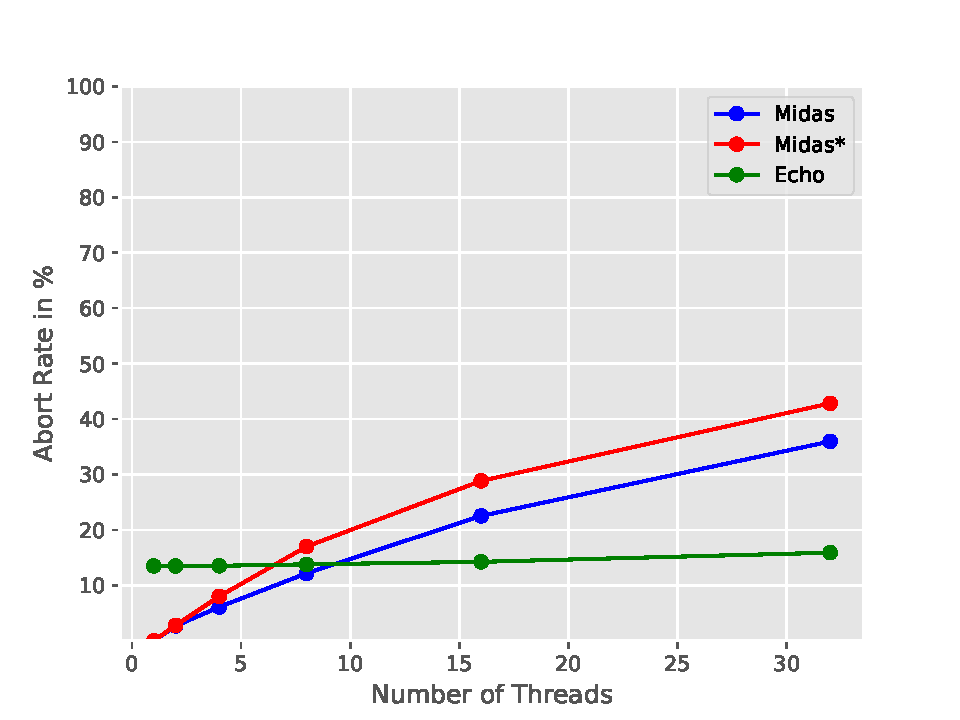
\includegraphics[width=\textwidth]{figures/bench/ar-ss}
    \caption{Abort rate for scenario S1.}
    \label{fig:ar-s1}
\end{minipage}
\end{figure}

%==============================================================================
% [2 = SL]
%==============================================================================

\paragraph{Scenario S2}

This scenario simulates a small database accessed by long transactions. It can
be seen as the worst-case scenario for concurrency controls with strong
isolation levels. As expected, transaction throughput of Midas suffers greatly
from the high contention as depicted in Figure \ref{fig:ttp-s2}. The reason is
that many threads spend a lot of time waiting at few critical sections and still
many conflicts do occur. As a result, speedup factor and parallel efficiency are
plummeting for all KVS (see Figures \ref{fig:spd-s2}, \ref{fig:eff-s2}). Still,
Midas performs significantly worse, which can be attributed to the higher number
of aborts due to serializability (see Figure \ref{fig:ar-s2}).

\begin{figure}[h!]
\begin{minipage}[l]{0.50\textwidth}
    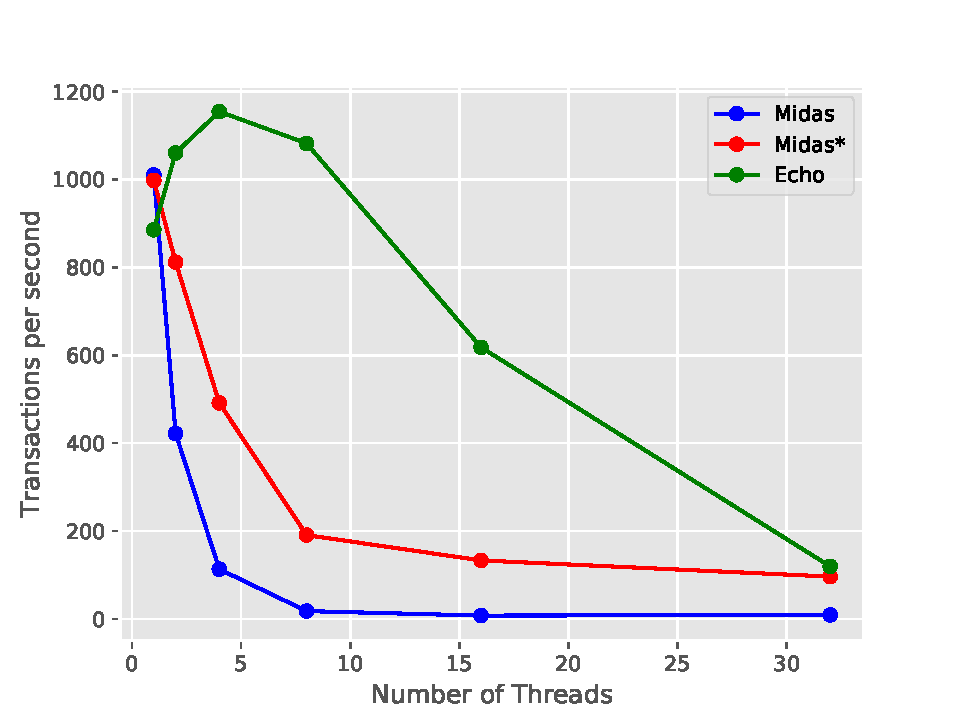
\includegraphics[width=\textwidth]{figures/bench/ttp-sl}
    \caption{Transaction throughput for\\scenario S2.}
    \label{fig:ttp-s2}
\end{minipage}
\begin{minipage}[l]{0.50\textwidth}
    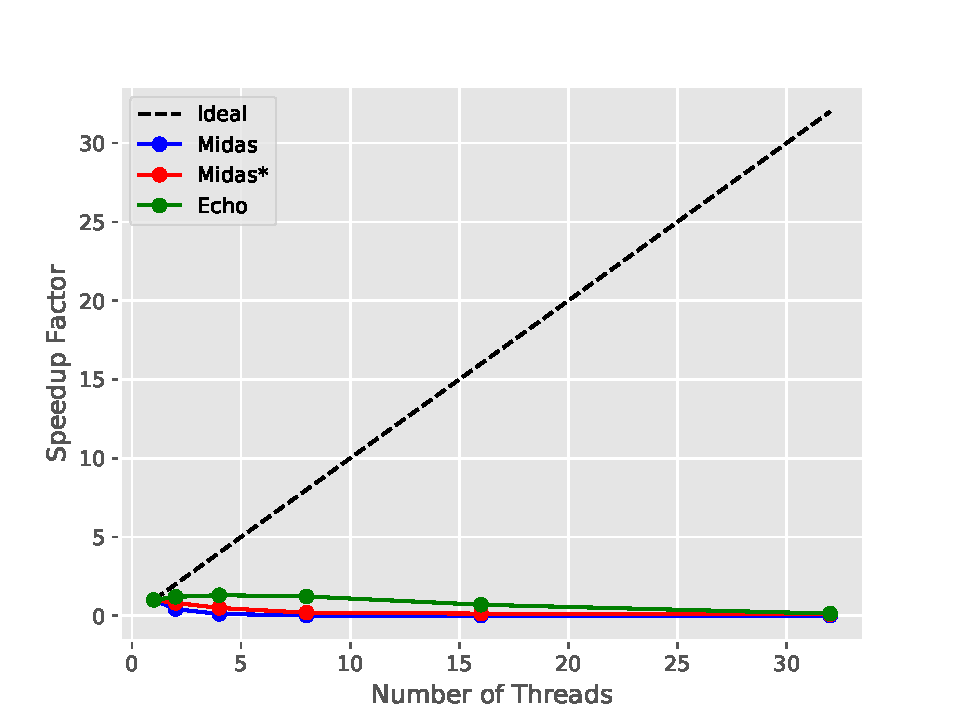
\includegraphics[width=\textwidth]{figures/bench/spd-sl}
    \caption{Transaction throughput speedup for scenario S2.}
    \label{fig:spd-s2}
\end{minipage}
\begin{minipage}[l]{0.50\textwidth}
    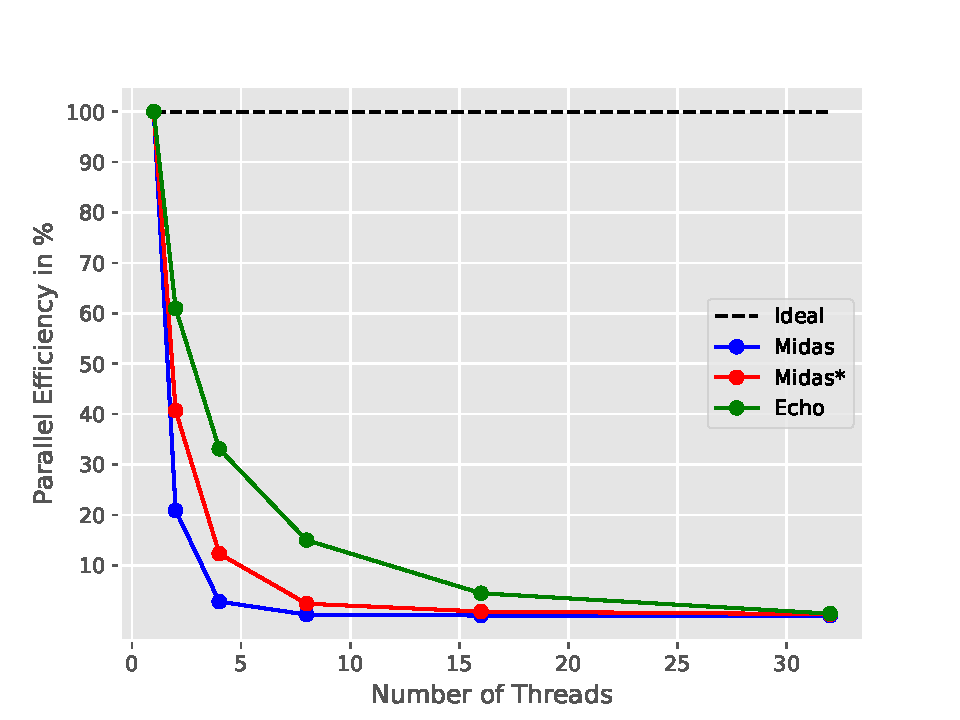
\includegraphics[width=\textwidth]{figures/bench/eff-sl}
    \caption{Parallel efficiency for scenario S2.}
    \label{fig:eff-s2}
\end{minipage}
\begin{minipage}[l]{0.50\textwidth}
    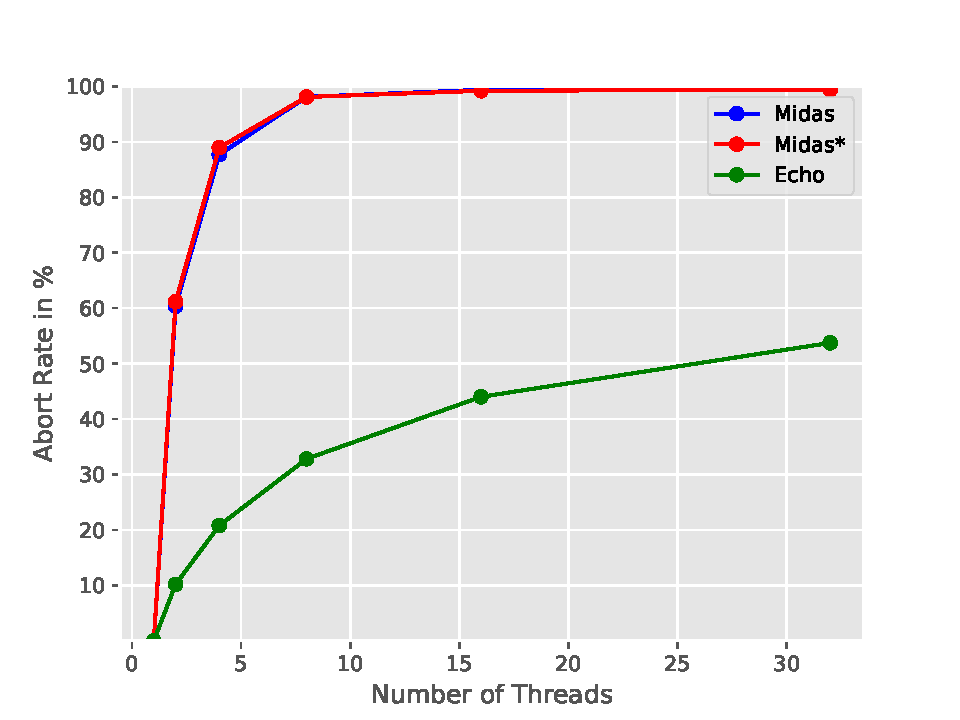
\includegraphics[width=\textwidth]{figures/bench/ar-sl}
    \caption{Abort rate for scenario S2.}
    \label{fig:ar-s2}
\end{minipage}
\end{figure}

%==============================================================================
% [3 = LS]
%==============================================================================

\todo[inline]{Are we talking about threads or cores? (most likely cores -> change captions in figures)}

\paragraph{Scenario S3}

This scenario simulates low contention through a large database and short
transactions. In this case, conflicts are rare which results in negligible abort
rates for all KVS, even with serializability (see Figure \ref{fig:ar-s3}). A
side effect is that throughput values are not distorted by time savings from
aborted transactions. While the original implementation of Midas fails to
improve throughput with additional cores, the optimized variant shows that the
overall concept of Midas works very well in low-contention scenarios (see
\ref{fig:spd-s3} and \ref{fig:eff-s3}). In particular, Midas$^{*}$ manages to
improve throughput up until 16 cores. Echo, on the other hand, scales worse as
speedup plummets for more than 8 cores. In terms of absolute throughput depicted
in Figure \ref{fig:ttp-s3}, Midas$^{*}$ manages to surpass Echo by a large
margin. This is a significant result, because non-serializable SI was adopted
for low-contention, read-mostly environments, in the first place. However, it
must be noted, that other factors may play a role in this. For instance, Echo
and Midas use different backends to handle potential NVRAM. Also, the optimized
variant of Midas does not synchronize access to its index, which is a very
optimistic approximation of a non-blocking concurrent implementation.

\begin{figure}[h!]
\begin{minipage}[l]{0.50\textwidth}
    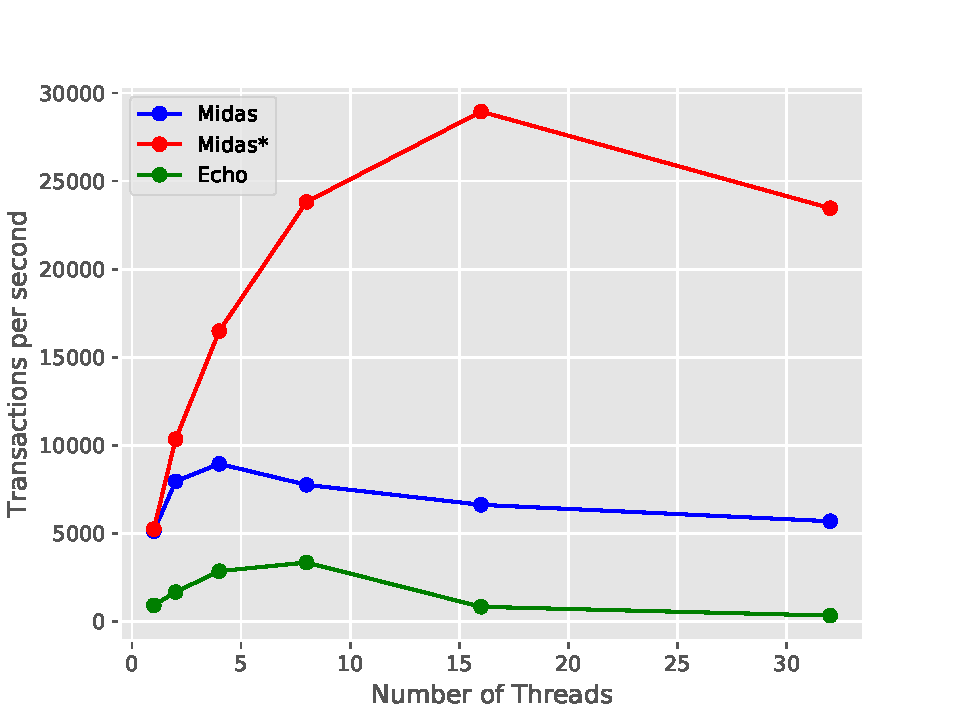
\includegraphics[width=\textwidth]{figures/bench/ttp-ls}
    \caption{Transaction throughput for\\scenario S3.}
    \label{fig:ttp-s3}
\end{minipage}
\begin{minipage}[l]{0.50\textwidth}
    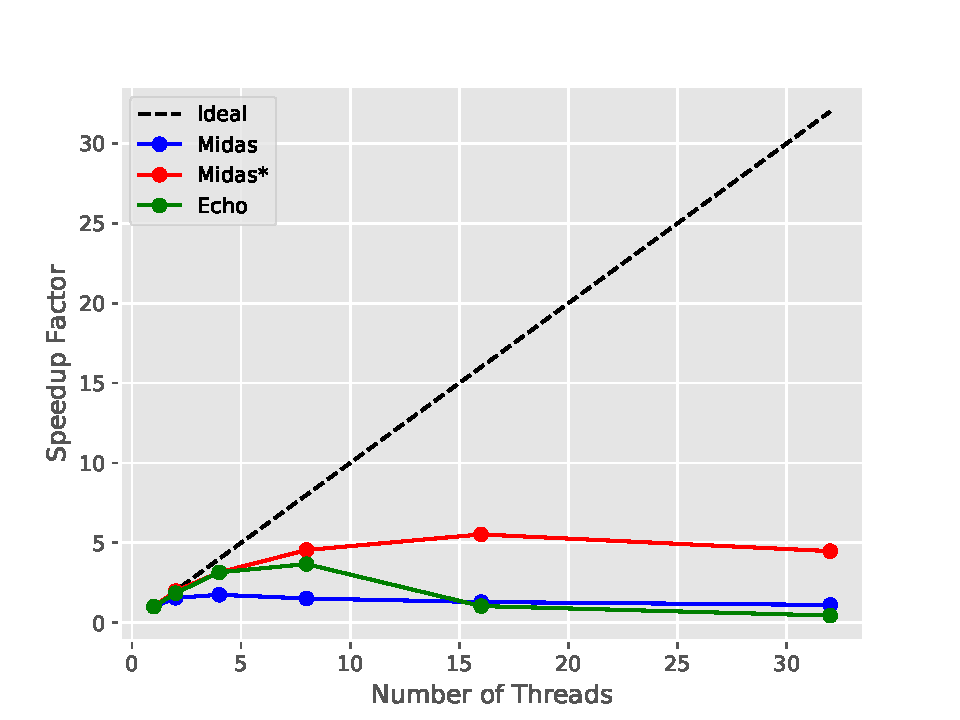
\includegraphics[width=\textwidth]{figures/bench/spd-ls}
    \caption{Transaction throughput speedup for scenario S3.}
    \label{fig:spd-s3}
\end{minipage}
\begin{minipage}[l]{0.50\textwidth}
    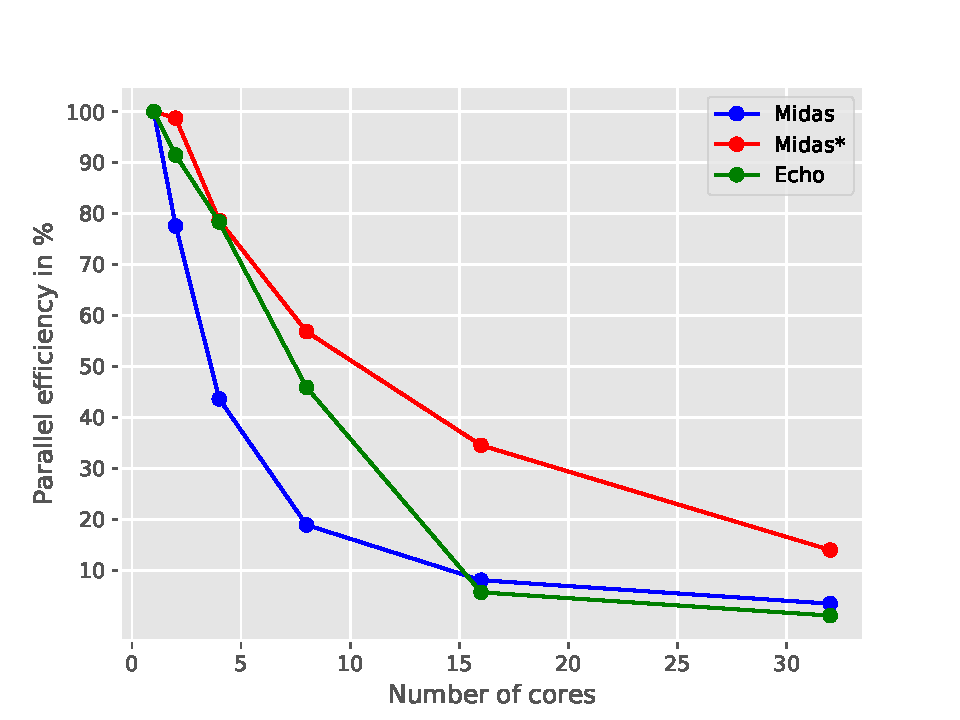
\includegraphics[width=\textwidth]{figures/bench/eff-ls}
    \caption{Parallel efficiency for scenario S3.}
    \label{fig:eff-s3}
\end{minipage}
\begin{minipage}[l]{0.50\textwidth}
    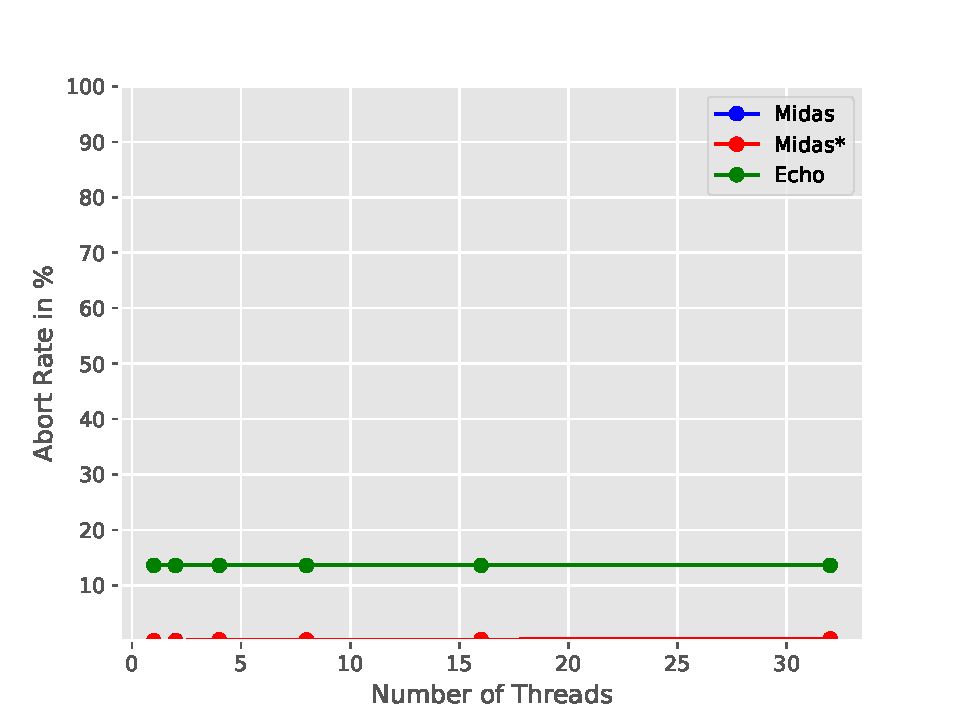
\includegraphics[width=\textwidth]{figures/bench/ar-ls}
    \caption{Abort rate for scenario S3.}
    \label{fig:ar-s3}
\end{minipage}
\end{figure}

%==============================================================================
% [4 = LL]
%==============================================================================

\paragraph{Scenario S4}

The last scenario simulates medium contention through a large database but long
transactions. As before, it can be seen in Figures \ref{fig:ttp-s4} through
\ref{fig:ar-s4}, that the first version of Midas fails to leverage additional
processors while abort rates increase. The optimized version performs much
better in terms of total throughput and speedup but also encounters even more
aborts. In fact, Figure \ref{fig:ar-s4} shows that, longer transactions alone
can cause abort rates to scale in the number of cores for both variants of
Midas. Also, starting beyond 16 cores, synchronization overhead in Midas$^{*}$
can no longer be compensated by time savings from aborted transactions (see
Figure \ref{fig:ttp-s4} and \ref{fig:spd-s4}). Echo, on the other hand, has
significantly fewer aborts but cannot leverage more than eight cores
efficiently. At the bottom line, even though Midas$^{*}$ has higher abort rates,
it performs and scales better in terms of transaction throughput than Echo.

\begin{figure}[h!]
\begin{minipage}[l]{0.50\textwidth}
    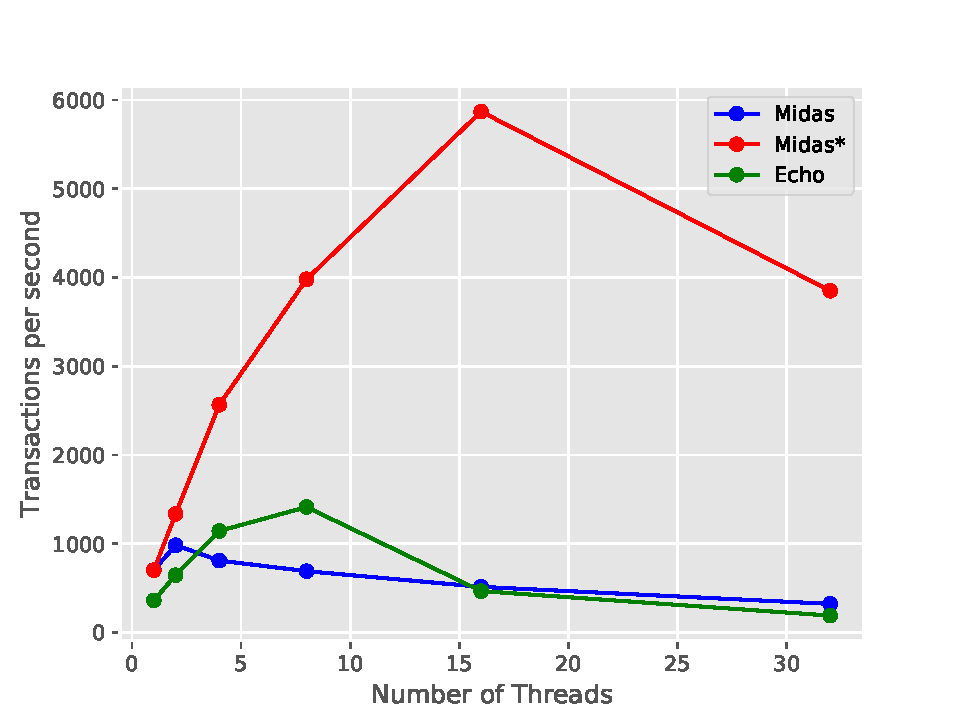
\includegraphics[width=\textwidth]{figures/bench/ttp-ll}
    \caption{Transaction throughput for\\scenario S4.}
    \label{fig:ttp-s4}
\end{minipage}
\begin{minipage}[l]{0.50\textwidth}
    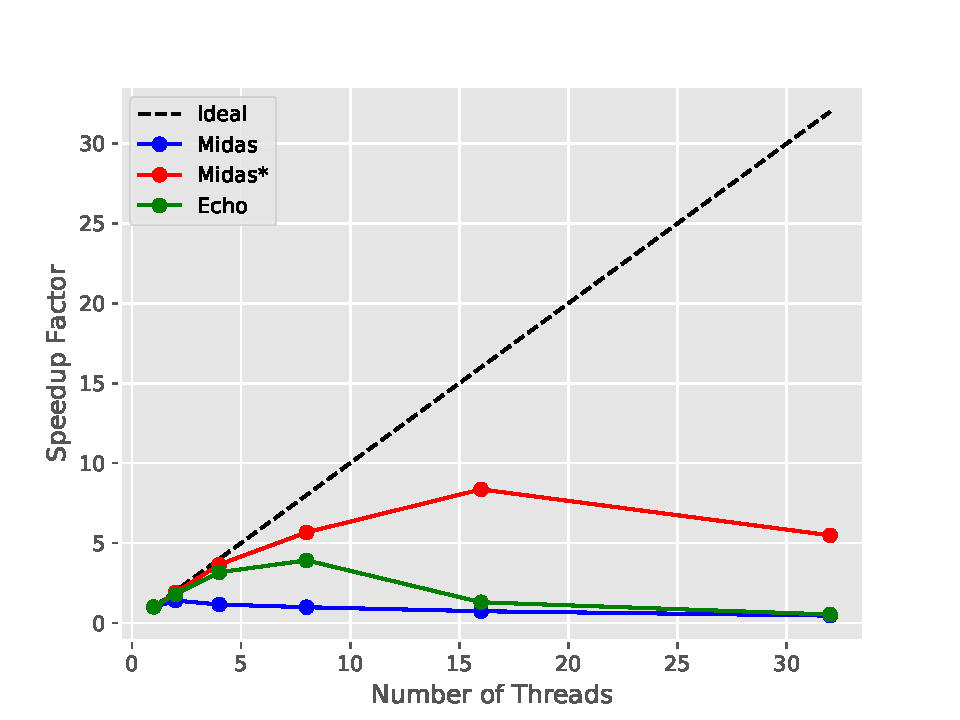
\includegraphics[width=\textwidth]{figures/bench/spd-ll}
    \caption{Transaction throughput speedup for scenario S4.}
    \label{fig:spd-s4}
\end{minipage}
\begin{minipage}[l]{0.50\textwidth}
    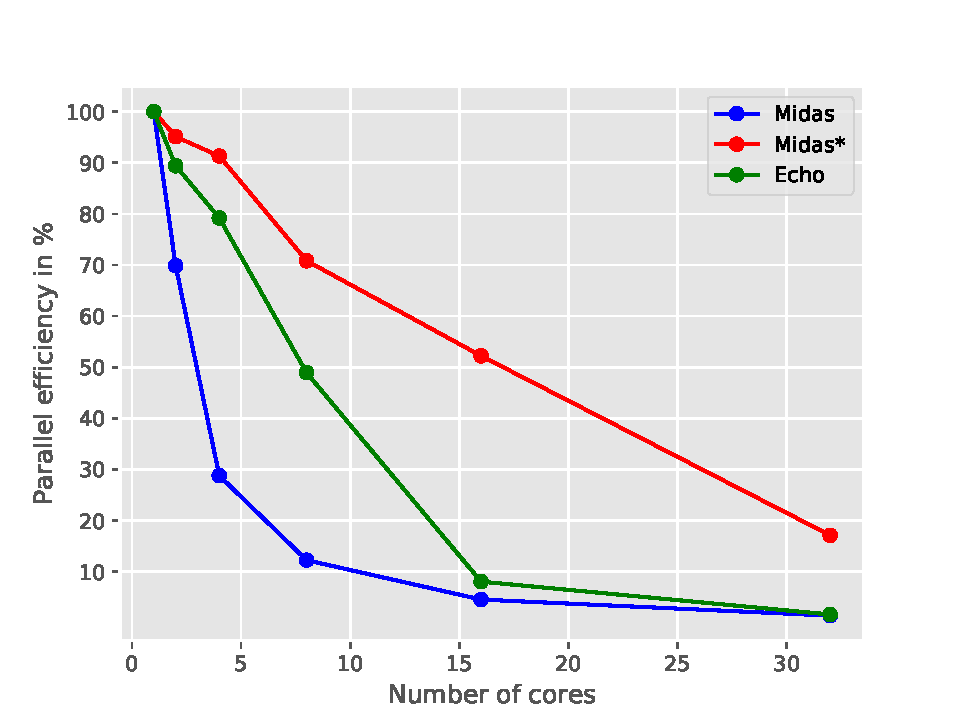
\includegraphics[width=\textwidth]{figures/bench/eff-ll}
    \caption{Parallel efficiency for scenario S4.}
    \label{fig:eff-s4}
\end{minipage}
\begin{minipage}[l]{0.50\textwidth}
    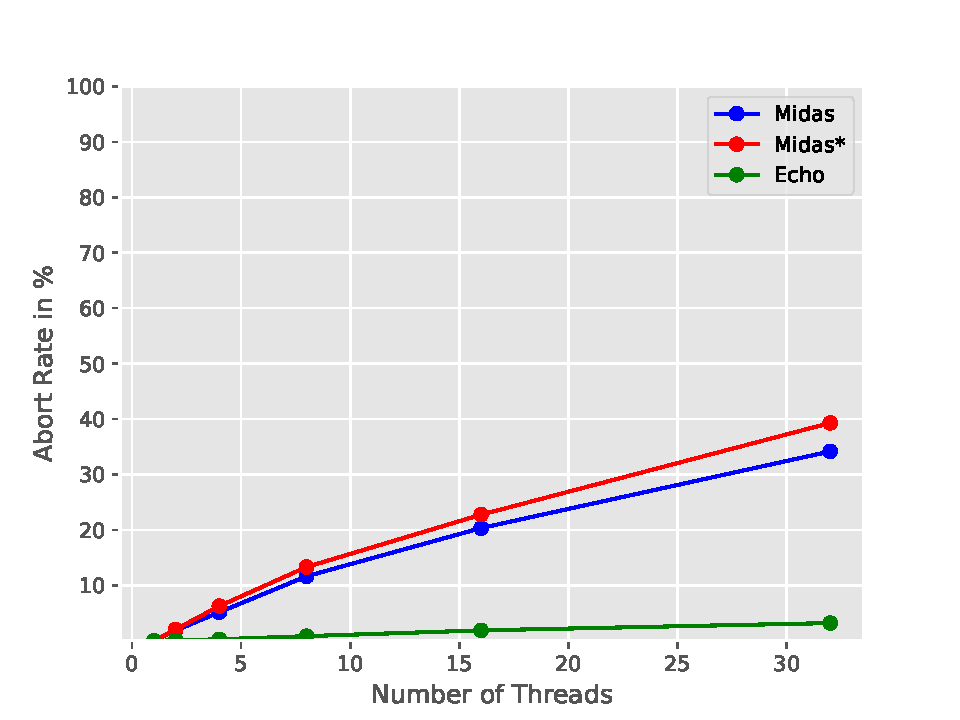
\includegraphics[width=\textwidth]{figures/bench/ar-ll}
    \caption{Abort rate for scenario S4.}
    \label{fig:ar-s4}
\end{minipage}
\end{figure}

\todo[inline]{Werden Captions mit Punkt beendet???}
